

\section*{K5/2. feladat: Szénacél csőre kifagyó jégréteg}
\addcontentsline{toc}{section}{K5/2. feladat: Szénacél csőre kifagyó jégréteg}

\begin{tabular}{ | p{2cm} | p{14cm} | } 
	\hline
	Név & Szalay István \\ 
	\hline
	Szak & \\ 
	\hline
	Félév & 2019/2020 II. (tavaszi) félév \\ 
	\hline
\end{tabular}
\vspace{0.5cm}

\noindent Egy NÁ125-ös szénacél csőben (a külső átmérő $d_2 = \SI{133}{\milli\meter}$, a belső átmérő $d_1 = \SI{125}{\milli\meter}$, a falvastagság $s = \SI{4}{\milli\meter}$) ammóniát szállítanak, amelynek nyomása $p = \SI{2.9}{\bar}$, hőmérséklete $T_1 = \SI{-10}{\celsius}$.

A környezet levegője ($T_4 = \SI{+10}{\celsius}$) melegíti a csövet, ammónia forrásban van a cső belsejében, így belülről hőelvonás van, és a cső hideg külső felületére kifagy a levegő nedvességtartalma. A kifagyott jégréteg szigetelőként működik, beáll az egyensúlyi állapot.

Meghatározandó a csőre fagyott jégréteg külső $d_3$ átmérője! A jégréteg felületének hőmérséklete $T_3 = \SI{0}{\celsius}$ (olvadó jég), a csőfal belső hőmérséklete pedig a forrásban lévő ammónia jó hőátadási tényezője miatt $T_1 = \SI{-10}{\celsius}$-nak vehető (a hőátadás termikus ellenállása elhanyagolható).

\begin{figure}[h]
	\centering
	\begin{tikzpicture}
		% Fiktív értékek a vázlathoz
		\pgfmathsetmacro{\DB}{4}
		\pgfmathsetmacro{\DK}{6}
		\pgfmathsetmacro{\DJ}{9}
		\pgfmathsetmacro{\lambdaA}{8}
		\pgfmathsetmacro{\lambdaJ}{2.9}
		\pgfmathsetmacro{\alfaL}{11.5}
		\pgfmathsetmacro{\qlin}{326.815}
		
		\pgfmathsetmacro{\RA}{\DB/2}
		\pgfmathsetmacro{\RB}{\DK/2}
		\pgfmathsetmacro{\RC}{\DJ/2}
		
		\pgfmathsetmacro{\L}{3}
		
		\pgfmathsetmacro{\kelvin}{4.2}
		\pgfmathsetmacro{\TA}{-10/\kelvin}
		\pgfmathsetmacro{\TB}{-7.36/\kelvin}
		\pgfmathsetmacro{\TC}{0/\kelvin}
		\pgfmathsetmacro{\TD}{10/\kelvin}
		
		% KÖRBEVÁGÁS
		\clip ({-1.25}, {-(\L)-2}) rectangle ({2.2*\RC}, {\L+1});
		
		% A csőfal és a jégréteg
		\fill[gray, opacity=0.25] (\RA,\L) -- ({(\RA+\RB)/2-0.16},\L) -- ({(\RA+\RB)/2-0.08}, {\L-0.12}) -- ({(\RA+\RB)/2+0.08}, {\L+0.12}) -- ({(\RA+\RB)/2+0.16}, \L) -- (\RB, \L) -- (\RB, -\L) -- ({(\RA+\RB)/2+0.16}, -\L) -- ({(\RA+\RB)/2+0.08}, {-\L+0.12}) -- ({(\RA+\RB)/2-0.08}, {-\L-0.12}) -- ({(\RA+\RB)/2-0.16},-\L) -- (\RA,-\L);
		\draw[] (\RA,\L) -- ({(\RA+\RB)/2-0.16},\L) -- ({(\RA+\RB)/2-0.08}, {\L-0.12}) -- ({(\RA+\RB)/2+0.08}, {\L+0.12}) -- ({(\RA+\RB)/2+0.16}, \L) -- (\RB, \L);
		\draw[] (\RA,-\L) -- ({(\RA+\RB)/2-0.16},-\L) -- ({(\RA+\RB)/2-0.08}, {-\L-0.12}) -- ({(\RA+\RB)/2+0.08}, {-\L+0.12}) -- ({(\RA+\RB)/2+0.16}, -\L) -- (\RB, -\L);
		
		\fill[blue, opacity=0.25] (\RB,\L) -- ({(\RB+\RC)/2-0.16},\L) -- ({(\RB+\RC)/2-0.08}, {\L-0.12}) -- ({(\RB+\RC)/2+0.08}, {\L+0.12}) -- ({(\RB+\RC)/2+0.16}, \L) -- (\RC, \L) -- (\RC, -\L) -- ({(\RB+\RC)/2+0.16}, -\L) -- ({(\RB+\RC)/2+0.08}, {-\L+0.12}) -- ({(\RB+\RC)/2-0.08}, {-\L-0.12}) -- ({(\RB+\RC)/2-0.16},-\L) -- (\RB,-\L);
		\draw[] (\RB,\L) -- ({(\RB+\RC)/2-0.16},\L) -- ({(\RB+\RC)/2-0.08}, {\L-0.12}) -- ({(\RB+\RC)/2+0.08}, {\L+0.12}) -- ({(\RB+\RC)/2+0.16}, \L) -- (\RC, \L);
		\draw[] (\RB,-\L) -- ({(\RB+\RC)/2-0.16},-\L) -- ({(\RB+\RC)/2-0.08}, {-\L-0.12}) -- ({(\RB+\RC)/2+0.08}, {-\L+0.12}) -- ({(\RB+\RC)/2+0.16}, -\L) -- (\RC, -\L);
		
		\draw[ultra thick] (\RA,-\L) -- (\RA,\L);
		\draw[ultra thick] (\RB,-\L) -- (\RB,\L);
		\draw[ultra thick] (\RC,-\L) -- (\RC,\L);
		
		% Tengelyek
		\draw[->] (0,-\L) -- (0,\L+1) node[anchor=north east]{$T$};
		\draw[->] (-1.25, 0) -- (\RC+3, 0) node[anchor=base east, shift={(0,-0.5)}]{$r$};
		
		% Hőáram és hőáramsűrűség
		\draw[->, ultra thick] (\RC-0.2,{\L+0.35}) -- ({(\RA+\RC)/2},{\L+0.35}) node[anchor=south]{$\dot{q}_{lin}$} -- (\RA+0.2,{\L+0.35});
		\draw[->, ultra thick] (\RC+2.2,{\L+0.35}) -- (\RC+1.2,{\L+0.35}) node[anchor=south]{$\dot{q}_{\acute{a}t}$} -- (\RC+0.2,{\L+0.35});
		
		% A hővezetési és hőátadási tényezők
		\node[anchor=base] at ({(\RA+\RB)/2},{\L-0.5}) {$\lambda_1$};
		\node[anchor=base] at ({(\RB+\RC)/2},{\L-0.5}) {$\lambda_2$};
		\node[anchor=base west] at ({(\RC+0.1},{\L-0.5}) {$\alpha$};
		
		% Az átmérők
		\pgflength[xa={-\RA}, ya={-\L}, xb={\RA}, yb={-\L}, alim=0, blim=1, ra=0.6]{$\diameter d_1$};
		\pgflength[xa={-\RB}, ya={-\L}, xb={\RB}, yb={-\L}, alim=0, blim=1, ra=1.2]{$\diameter d_2$};
		\pgflength[xa={-\RC}, ya={-\L}, xb={\RC}, yb={-\L}, alim=0, blim=1, ra=1.8]{$\diameter d_3$};
		
		% T(r) körülbelüli hőmérséklet-hely függvény
		\draw[red, ultra thick] (0.5,\TA) -- (\RA,\TA);
		\draw[ultra thick, color=red, domain=\RA:\RB, smooth, variable=\r] plot (\r, {\TA + ( \qlin/(2*3.14159*\lambdaA) * ln(2*\r/\DB))/\kelvin});
		\draw[ultra thick, color=red, domain=\RB:\RC, smooth, variable=\r] plot (\r, {\TA + (\qlin/(2*3.14159*\lambdaA) * ln(\DK/\DB) + \qlin/(2*3.14159*\lambdaJ) * ln(2*\r/\DK))/\kelvin});
		
		\draw[ultra thick, color=red, domain=\RC:1.5*\RC, smooth, variable=\r] plot (\r, {\TD * (1-exp(-(\r-\RC)/0.5))});
		
		% A hőmérséklet értékek
		\draw (-0.1,\TA) -- (0.1,\TA);
		\node[anchor=base east] at (0,\TA) {$T_1$};
		\node[anchor=north east] at (0,\TA) {$\SI{-10}{\celsius}$};
		
		\draw (-0.1,\TB) -- (0.1,\TB);
		\draw[black, opacity=0.5, dashed] (0,\TB) -- (\RB,\TB);
		\node[anchor=base east] at (0,\TB) {$T_2$};
		
		\draw (-0.1,\TD) -- (0.1,\TD);
		\draw[black, opacity=0.5, dashed] (0,\TD) -- (1.5*\RC,\TD);
		\node[anchor=base east] at (0,\TD) {$T_4$};
		\node[anchor=north east] at (0,\TD) {$\SI{10}{\celsius}$};
		
		\node[anchor=north west] at (\RC,\TC) {$T_3$};
		\node[anchor=north west] at (\RC, -0.45) {$\SI{0}{\celsius}$};
		
		% Feliratok
		\node[anchor=base east] at (\RA, \L) {ammónia};
		\node[anchor=base west] at (\RC, -\L) {levegő};
		
		% Adatok
		\node[anchor=base west] at (1.6*\RC, \L) {$\lambda_1 = \SI{45}{\watt\per\meter\kelvin}$};
		\node[anchor=base west] at (1.6*\RC, 0.65*\L) {$\lambda_2 = \SI{2.32}{\watt\per\meter\kelvin}$};
		\node[anchor=base west] at (1.6*\RC, 0.3*\L) {$\alpha = \SI{11.5}{\watt\per\meter\squared\kelvin}$};
		
	\end{tikzpicture}
	\caption{A hőmérséklet-hely függvény \textbf{nem méretarányos} vázlata.}
\end{figure}

\subsubsection*{Vizsgálat többrétegű hengeres falként}
A csőfal és a rárakódó jégréteg hengeres alakú, ezért lineáris a hőáramsűrűségeket tudjuk felírni. A csőfalban és a jégrétegben állandósult a hőmérsékleteloszlás és csak hővezetés történik. A hengeres falakra a $\dot{q}_{lin}$ \textbf{vezetéses} lineáris hőáramsűrűség vonatkozik.
\begin{equation}
	\dot{q}_{lin} = \dfrac{T_3 - T_1}{\dfrac{\ln\frac{d_2}{d_1}}{2 \pi \lambda_1} + \dfrac{\ln\frac{d_3}{d_2}}{2 \pi \lambda_2}}
\end{equation}

A levegőből a jégrétegbe \textbf{átadódó} $\dot{q}_{\acute{a}t}$ lineáris hőáramsűrűség: 
\begin{equation}
	\dot{q}_{\acute{a}t} = \alpha d_3 \pi (T_4 - T_3)
\end{equation}

A két lineáris hőáramsűrűséget az ábrán úgy vettük fel, hogy a hőmérsékletcsökkenés irányába pozitívak, ezért a felírásuknál a nagyobb hőmérsékletből vonjuk ki a kisebbet.

Az energiamegmaradás miatt a két lineáris hőáramsűrűség egyenlő:
\begin{equation}
	\dot{q}_{lin} = \dot{q}_{\acute{a}t} = \dot{q}
\end{equation}

A fentiekből az alábbi kétismeretlenes egyenletrendszert kapjuk, amiben a jégréteg $d_3$ átmérője a a $\dot{q}$ lineáris hőáramsűrűség az ismeretlenek. Az egyenletrendszer nem lineáris, átrendezéssel nem oldható meg (transzcendens), csak numerikus közelítő megoldása lehetséges:
\begin{equation}
	\left.
	\begin{array}{lcl}
		\dot{q} = \dfrac{T_3 - T_1}{\dfrac{\ln\frac{d_2}{d_1}}{2 \pi \lambda_1} + \dfrac{\ln\frac{d_3}{d_2}}{2 \pi \lambda_2}} \\ \\
		\dot{q} = \alpha d_3 \pi (T_4 - T_3)
	\end{array}
	\right\rbrace
	\quad \Rightarrow \quad 
	\left\lbrace
	\begin{array}{lcl}
		\dot{q} \approx \SI{137.873}{\watt\per\meter} \\ \\
		d_3 \approx \SI{381.6}{\milli\meter}
	\end{array}
	\right.
\end{equation}

Innen a jégréteg vastagsága $\dfrac{1}{2}\left(d_3 - d_2\right) = \SI{124.3}{\milli\meter}$.

\subsubsection*{A méretarányos ábra és a hőmérséklet hely függvény}
A lineáris hőáramsűrűség és a jég külső átmérőjének numerikus közelítő megoldását felhasználva megrajzolható méretarányosan a $T\!\left(r\right)$ hőmérséklet-hely függvény. A hőmérséklet a $d_1$ átmérőn belül állandó $T_1$ érték. A csőfalban és a jégrétegben $T\!\left(r\right) = T_0 + \dfrac{\dot{q}}{2 \pi \lambda} \ln\dfrac{r}{r_0}$ alakban írható fel, ahol a $T_0$ a belső $r_0$ sugárhoz tartozó hőmérséklet.

A csőfal esetén $T_0 = T_1$ és $r_0 = \dfrac{d_1}{2}$:
\begin{equation}
	T\!\left(r\right) = T_1 + \dfrac{\dot{q}}{2 \pi \lambda_1} \ln\dfrac{2 r}{d_1}
\end{equation}

Innen megkaphatjuk a csőfal és a jégréteg határfelületének hőmértékletét, $T_2$-t:
\begin{equation}
	T_2 = T\!\left(\frac{d_2}{2}\right) = T_1 + \dfrac{\dot{q}}{2 \pi \lambda_1} \ln\dfrac{d_2}{d_1} = \SI{-9.96}{\celsius}
\end{equation}

A jégréteg esetén $T_0 = T_2$ és $r_0 = \dfrac{d_2}{2}$:
\begin{equation}
	T\!\left(r\right) = T_2 + \dfrac{\dot{q}}{2 \pi \lambda_2} \ln\dfrac{2 r}{d_2}
\end{equation}


\begin{figure}[h]
	\centering
	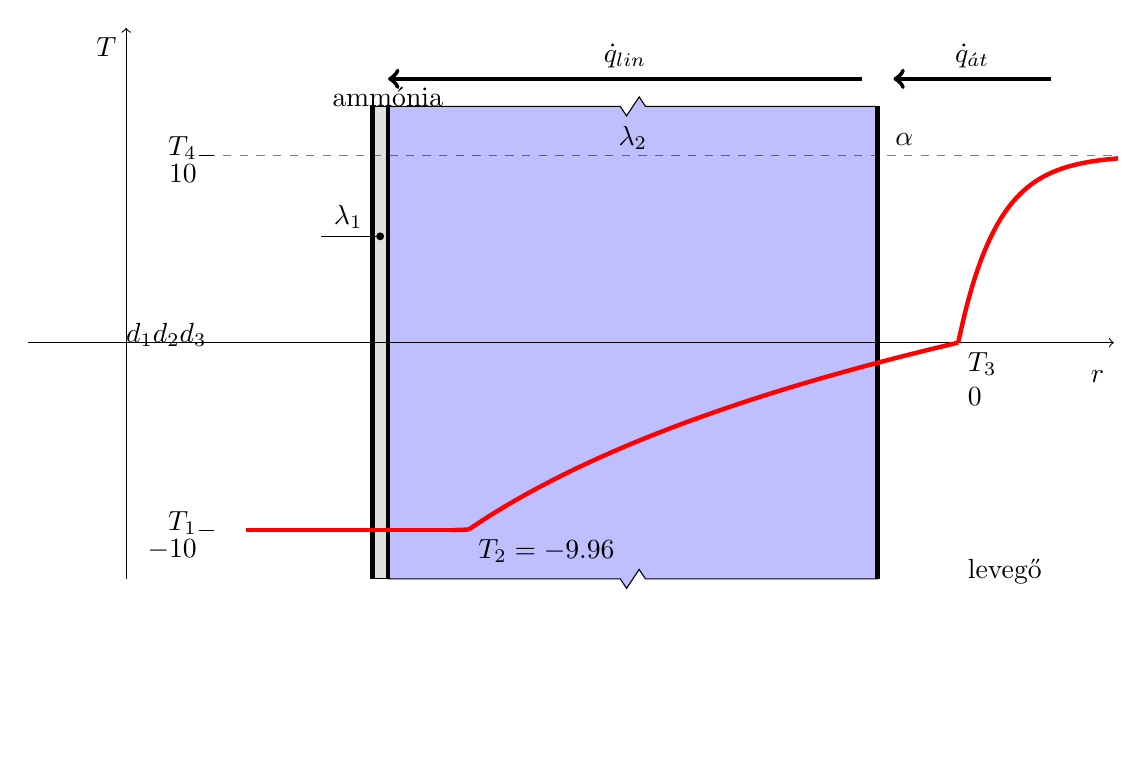
\begin{tikzpicture}
		% Fiktív értékek a vázlathoz
		\pgfmathsetmacro{\meter}{1/50}
		\pgfmathsetmacro{\DB}{0.125/\meter}
		\pgfmathsetmacro{\DK}{0.133/\meter}
		\pgfmathsetmacro{\DJ}{0.3816/\meter}
		\pgfmathsetmacro{\lambdaA}{45}
		\pgfmathsetmacro{\lambdaJ}{2.32}
		\pgfmathsetmacro{\alfaL}{11.5}
		\pgfmathsetmacro{\qlin}{137.873}
		
		\pgfmathsetmacro{\RA}{\DB/2}
		\pgfmathsetmacro{\RB}{\DK/2}
		\pgfmathsetmacro{\RC}{\DJ/2}
		
		\pgfmathsetmacro{\L}{3}
		
		\pgfmathsetmacro{\kelvin}{4.2}
		\pgfmathsetmacro{\TA}{-10/\kelvin}
		\pgfmathsetmacro{\TB}{-9.96/\kelvin}
		\pgfmathsetmacro{\TC}{0/\kelvin}
		\pgfmathsetmacro{\TD}{10/\kelvin}
		
		% KÖRBEVÁGÁS
		\clip ({-1.25}, {-(\L)-2}) rectangle ({1.32*\RC}, {\L+1});
		
		% A csőfal és a jégréteg
		\fill[gray,opacity=0.25] (\RA,\L) -- (\RB, \L) -- (\RB, -\L) -- (\RA,-\L);
		\draw[] (\RA,\L) -- (\RB, \L);
		\draw[] (\RA,-\L) -- (\RB, -\L);
		
		\fill[blue,opacity=0.25] (\RB,\L) -- ({(\RB+\RC)/2-0.16},\L) -- ({(\RB+\RC)/2-0.08}, {\L-0.12}) -- ({(\RB+\RC)/2+0.08}, {\L+0.12}) -- ({(\RB+\RC)/2+0.16}, \L) -- (\RC, \L) -- (\RC, -\L) -- ({(\RB+\RC)/2+0.16}, -\L) -- ({(\RB+\RC)/2+0.08}, {-\L+0.12}) -- ({(\RB+\RC)/2-0.08}, {-\L-0.12}) -- ({(\RB+\RC)/2-0.16},-\L) -- (\RB,-\L);
		\draw[] (\RB,\L) -- ({(\RB+\RC)/2-0.16},\L) -- ({(\RB+\RC)/2-0.08}, {\L-0.12}) -- ({(\RB+\RC)/2+0.08}, {\L+0.12}) -- ({(\RB+\RC)/2+0.16}, \L) -- (\RC, \L);
		\draw[] (\RB,-\L) -- ({(\RB+\RC)/2-0.16},-\L) -- ({(\RB+\RC)/2-0.08}, {-\L-0.12}) -- ({(\RB+\RC)/2+0.08}, {-\L+0.12}) -- ({(\RB+\RC)/2+0.16}, -\L) -- (\RC, -\L);
		
		\draw[ultra thick] (\RA,-\L) -- (\RA,\L);
		\draw[ultra thick] (\RB,-\L) -- (\RB,\L);
		\draw[ultra thick] (\RC,-\L) -- (\RC,\L);
		
		% Tengelyek
		\draw[->] (0,-\L) -- (0,\L+1) node[anchor=north east]{$T$};
		\draw[->] (-1.25, 0) -- (\RC+3, 0) node[anchor=base east, shift={(0,-0.5)}]{$r$};
		
		% Hőáram és hőáramsűrűség
		\draw[->, ultra thick] (\RC-0.2,{\L+0.35}) -- ({(\RA+\RC)/2},{\L+0.35}) node[anchor=south]{$\dot{q}_{lin}$} -- (\RA+0.2,{\L+0.35});
		\draw[->, ultra thick] (\RC+2.2,{\L+0.35}) -- (\RC+1.2,{\L+0.35}) node[anchor=south]{$\dot{q}_{\acute{a}t}$} -- (\RC+0.2,{\L+0.35});
		
		% A hővezetési és hőátadási tényezők
		\node[anchor=base east] at ({\RA},{\L-1.5}) {$\lambda_1$};
		\draw ({\RA-0.65},{\L-1.65}) -- ({(\RA+\RB)/2},{\L-1.65});
		\fill[] ({(\RA+\RB)/2},{\L-1.65}) circle[radius=0.05];
		
		\node[anchor=base] at ({(\RB+\RC)/2},{\L-0.5}) {$\lambda_2$};
		\node[anchor=base west] at ({(\RC+0.1},{\L-0.5}) {$\alpha$};
		
		% Az átmérők
		\pgflength[xa={-\RA}, ya={-\L}, xb={\RA}, yb={-\L}, alim=0, blim=1, ra=0.6]{$\diameter d_1$};
		\pgflength[xa={-\RB}, ya={-\L}, xb={\RB}, yb={-\L}, alim=0, blim=1, ra=1.2]{$\diameter d_2$};
		\pgflength[xa={-\RC}, ya={-\L}, xb={\RC}, yb={-\L}, alim=0, blim=1, ra=1.8]{$\diameter d_3$};
		
		% A T(r) VALÓS hőmérséklet-hely függvény
		\draw[red, ultra thick] (0.5,\TA) -- (\RA,\TA);
		
		\draw[ultra thick, color=red, domain=\RA:\RB, smooth, variable=\r] plot (\r, {\TA + ( \qlin/(2*3.14159*\lambdaA) * ln(2*\r/\DB))/\kelvin});
		
		\draw[ultra thick, color=red, domain=\RB:\RC, smooth, variable=\r] plot (\r, {\TA + (\qlin/(2*3.14159*\lambdaA) * ln(\DK/\DB) + \qlin/(2*3.14159*\lambdaJ) * ln(2*\r/\DK))/\kelvin});
		
		\draw[ultra thick, color=red, domain=\RC:1.25*\RC, smooth, variable=\r] plot (\r, {\TD * (1-exp(-(\r-\RC)/0.5))});
		
		% A hőmérséklet értékek
		\draw (-0.1,\TA) -- (0.1,\TA);
		\node[anchor=base east] at (0,\TA) {$T_1$};
		\node[anchor=north east] at (0,\TA) {$\SI{-10}{\celsius}$};
		
		\node[anchor=north west] at (\RB,\TB) {$T_2 = \SI{-9.96}{\celsius}$};
		
		\draw (-0.1,\TD) -- (0.1,\TD);
		\draw[black, opacity=0.5, dashed] (0,\TD) -- (1.25*\RC,\TD);
		\node[anchor=base east] at (0,\TD) {$T_4$};
		\node[anchor=north east] at (0,\TD) {$\SI{10}{\celsius}$};
		
		\node[anchor=north west] at (\RC,\TC) {$T_3$};
		\node[anchor=north west] at (\RC, -0.45) {$\SI{0}{\celsius}$};
		
		% Feliratok
		\node[anchor=base east] at (\RA, \L) {ammónia};
		\node[anchor=base west] at (\RC, -\L) {levegő};
		
	\end{tikzpicture}
	\caption{A hőmérséklet-hely függvény méretarányosan ábrázolva.}
\end{figure}


\subsubsection*{Vizsgálat többrétegű síkfalként}
A hengeres falon keresztül történő hőterjedés mindig közelíthető a hengeres fal kiterítésével kapott síkfalon át történő hőterjedéssel. A közelítés hibája a a hengeres fal vastagságától függ, minél vékonyabb, annál kisebb a síkfallal történő közelítés hibája.

A többrétegű hengeres falat többrétegű síkfallal közelíthetjük. A közelítő síkfal vastagsága és hossza megegyezik a hengeres réteg vastagságával és hosszával, a szélessége a hengeres réteg közepes átmérőjéhez tartozó kerülettel közelíthető:
\begin{equation}
	\left.
	\begin{array}{l}
		\dot{q}_{lin} = \dfrac{\lambda_1}{\frac{d_2-d_1}{2}} \dfrac{d_1+d_2}{2} \pi (T_2 - T_1) \\ \\
		\dot{q}_{lin} = \dfrac{\lambda_2}{\frac{d_3-d_2}{2}} \dfrac{d_2+d_3}{2} \pi (T_3 - T_2)
	\end{array}
	\right\rbrace
	\quad \Rightarrow \quad 
	\dot{q}_{lin} = \dfrac{T_3 - T_1}{
		\dfrac{d_2-d_1}{\lambda_1\left(d_1+d_2\right) \pi} + 
		\dfrac{d_3-d_2}{\lambda_2\left(d_2+d_3\right) \pi}
		}
\end{equation}

A falbeli lineáris hőáram és a hőátadást jellemző lineáris hőáram most is egyenlő. 
\begin{equation}
	\dot{q}_{lin} = \dfrac{T_3 - T_1}{
		\dfrac{d_2-d_1}{\lambda_1\left(d_1+d_2\right) \bcancel{\pi}} + 
		\dfrac{d_3-d_2}{\lambda_2\left(d_2+d_3\right)\bcancel{\pi}}
		}
	= 
	\alpha d_3 \bcancel{\pi} (T_4 - T_3) = \dot{q}_{\acute{a}t}
\end{equation}

Egyszerűsítve, és kifejezve a hőmérsékletkülönbségek hányadosát:
\begin{equation}
	\underbrace{\dfrac{T_3 - T_1}{T_4 - T_3}}_{\substack{T \\ \text{állandó}}}
	= 
	\underbrace{\dfrac{\left(d_2-d_1\right)\alpha}{\lambda_1\left(d_1+d_2\right)}}_{\substack{C \\ \text{állandó}}} d_3
	+ 
	\dfrac{\left(d_3-d_2\right) \alpha d_3}{\lambda_2\left(d_2+d_3\right)}
\end{equation}

Vezessük be a $T$ és $C$ állandókat, hogy gyorsabb és átláthatóbb legyen az egyenlet átrendezése:
\begin{equation}
	T = C d_3 +  \dfrac{\left(d_3-d_2\right) \alpha d_3}{\lambda_2\left(d_2+d_3\right)}
\end{equation}

Megszüntetve a törtet $d_3$-ra másodfokú egyenletet kapunk:
\begin{equation}
	T \lambda_2\left(d_2+d_3\right) = C d_3 \lambda_2\left(d_2+d_3\right) + \left(d_3-d_2\right) \alpha d_3
\end{equation}

\begin{equation}
	\SI{0}{\watt} = \left(C \lambda_2 +\alpha\right)d_3^2 + \left(C \lambda_2 d_2 - d_2 \alpha - T \lambda_2 \right) d_3 - T \lambda_2 d_2
\end{equation}

Innen a $d_3$ közelítő értéke:
\begin{equation}
	d_{3,1} = \SI{0.4008}{\meter}, 
	\quad 
	\underbrace{
		\left(d_{3,2} = \SI{-0.0668}{\meter}\right)
	}_{\substack{\text{a másodfokú egyenletnek megoldása,} \\ \text{de a fizikai problémának nem}}}
\end{equation}

A $d_3$ közelítő megoldással nyert értéke tehát \SI{400.8}{\milli\meter}. A nemlineáris egyenlet közelítő numerikus megoldásától ez 5\,\%-kal tér el.

\pagebreak